 \let\negmedspace\undefined
\let\negthickspace\undefined
\documentclass[journal]{IEEEtran}
\usepackage[a5paper, margin=10mm, onecolumn]{geometry}
\usepackage{lmodern} % Ensure lmodern is loaded for pdflatex
\usepackage{tfrupee} % Include tfrupee package

\setlength{\headheight}{1cm} % Set the height of the header box
\setlength{\headsep}{0mm}     % Set the distance between the header box and the top of the text

\usepackage{gvv-book}
\usepackage{gvv}
\usepackage{cite}
\usepackage{amsmath,amssymb,amsfonts,amsthm}
\usepackage{algorithmic}
\usepackage{graphicx}
\usepackage{textcomp}
\usepackage{xcolor}
\usepackage{txfonts}
\usepackage{listings}
\usepackage{enumitem}
\usepackage{mathtools}
\usepackage{gensymb}
\usepackage{comment}
\usepackage[breaklinks=true]{hyperref}
\usepackage{tkz-euclide} 
\usepackage{listings}                                      
\def\inputGnumericTable{}                                 
\usepackage[latin1]{inputenc}                                
\usepackage{color}                                            
\usepackage{array}                                            
\usepackage{longtable}
\usepackage{multicol}
\usepackage{calc}                                             
\usepackage{multirow}                                         
\usepackage{hhline}                                           
\usepackage{ifthen}                                           
\usepackage{lscape}
\begin{document}
	
	\bibliographystyle{IEEEtran}
	\vspace{3cm}
	
	\title{6.5.25}
	\author{EE24BTECH11008 - Aslin Garvasis}
	% \maketitle
	% \newpage
	% \bigskip
	{\let\newpage\relax\maketitle}
	
	\renewcommand{\thefigure}{\theenumi}
	\renewcommand{\thetable}{\theenumi}
	\setlength{\intextsep}{10pt} % Space between text and floats
	
	
	\numberwithin{equation}{enumi}
	\numberwithin{figure}{enumi}
	\renewcommand{\thetable}{\theenumi}
	
	
	\textbf{Question}:\newline
	Show that the semi-vertical angle of the cone of the maximum volume and of given slant height is $\tan^{-1}\sqrt{2}$ \\
	


\section*{Solution (Classical Method)}

The volume \( V \) of a cone is given by the formula:

\begin{align}
V &= \frac{1}{3} \pi r^2 h
\end{align}

where:
- \( r \) is the radius of the base,
- \( h \) is the height of the cone.

The slant height \( l \) is related to the radius \( r \) and height \( h \) by the Pythagorean theorem:

\begin{align}
l^2 &= r^2 + h^2
\end{align}

Thus, the height \( h \) can be expressed as:

\begin{align}
h &= \sqrt{l^2 - r^2}
\end{align}

Substituting \( h = \sqrt{l^2 - r^2} \) into the volume formula, we get:

\begin{align}
V(r) &= \frac{1}{3} \pi r^2 \sqrt{l^2 - r^2}
\end{align}

To maximize the volume, we differentiate \( V(r) \) with respect to \( r \). First, we use the product and chain rules to find the derivative:

\begin{align}
\frac{dV}{dr} &= \frac{1}{3} \pi \left( 2r \sqrt{l^2 - r^2} + r^2 \cdot \frac{-r}{\sqrt{l^2 - r^2}} \right)
\end{align}

Simplifying, we have:

\begin{align}
\frac{dV}{dr} &= \frac{1}{3} \pi \left( 2r \sqrt{l^2 - r^2} - \frac{r^3}{\sqrt{l^2 - r^2}} \right)
\end{align}

We set \( \frac{dV}{dr} = 0 \) to find the critical points:

\begin{align}
2r \sqrt{l^2 - r^2} &= \frac{r^3}{\sqrt{l^2 - r^2}}
\end{align}

Multiplying both sides by \( \sqrt{l^2 - r^2} \), we obtain:

\begin{align}
2r (l^2 - r^2) &= r^3
\end{align}

Canceling \( r \) from both sides (assuming \( r \neq 0 \)):

\begin{align}
2(l^2 - r^2) &= r^2
\end{align}

Simplifying:

\begin{align}
2l^2 - 2r^2 &= r^2
\end{align}

\begin{align}
2l^2 &= 3r^2
\end{align}

Solving for \( r^2 \), we get:

\begin{align}
r^2 &= \frac{2}{3} l^2
\end{align}

Thus, the radius is:

\begin{align}
r &= \frac{\sqrt{2}}{\sqrt{3}} l
\end{align}

Now, we use the formula for the semi-vertical angle \( \theta \), which is given by:

\begin{align}
\tan(\theta) &= \frac{r}{h}
\end{align}

We substitute \( r = \frac{\sqrt{2}}{\sqrt{3}} l \) and calculate \( h \). From the relation \( l^2 = r^2 + h^2 \), we have:

\begin{align}
h &= \sqrt{l^2 - r^2} = \sqrt{l^2 - \frac{2}{3} l^2} = \sqrt{\frac{1}{3} l^2} = \frac{l}{\sqrt{3}}
\end{align}

Thus, \( \tan(\theta) \) becomes:

\begin{align}
\tan(\theta) &= \frac{\frac{\sqrt{2}}{\sqrt{3}} l}{\frac{l}{\sqrt{3}}} = \sqrt{2}
\end{align}

Therefore, the semi-vertical angle \( \theta \) is:

\begin{align}
\theta &= \tan^{-1}(\sqrt{2})
\end{align}

Hence, we have shown that the semi-vertical angle of the cone of maximum volume, given a fixed slant height, is:

\begin{align}
\boxed{\theta = \tan^{-1}(\sqrt{2})}
\end{align}
\\ \\

\section*{Solution (Gradient Descent Method)}

We will now solve the problem using the gradient descent method. We want to maximize the volume \( V(r) \) of the cone, which is given by:

\begin{align}
V(r) &= \frac{1}{3} \pi r^2 \sqrt{l^2 - r^2}
\end{align}

To do so, we use the gradient descent algorithm to iteratively find the value of \( r \) that maximizes the volume.

\subsection*{Step 1: Gradient of the Volume Function}

The gradient (derivative) of the volume with respect to \( r \) is:

\begin{align}
\frac{dV}{dr} &= \frac{1}{3} \pi \left( 2r \sqrt{l^2 - r^2} - \frac{r^3}{\sqrt{l^2 - r^2}} \right)
\end{align}

This is the function we will use for gradient descent.

\subsection*{Step 2: Iterative Update Rule}

In gradient descent, we update the variable \( r \) iteratively using the following rule:

\begin{align}
r_{n+1} &= r_n - \alpha \frac{dV}{dr}(r_n)
\end{align}

where \( \alpha \) is the learning rate, and \( r_n \) is the current value of \( r \).

\subsection*{Step 3: Choosing an Initial Guess}

We start with an initial guess for \( r \), say \( r_0 = \frac{l}{2} \), and choose a small learning rate \( \alpha \), for example \( \alpha = 0.01 \).

\subsection*{Step 4: Convergence Criterion}

We iterate the update rule until the change in volume is sufficiently small, i.e., when \( \left| r_{n+1} - r_n \right| < \epsilon \), where \( \epsilon \) is a small threshold (e.g., \( \epsilon = 10^{-6} \)).

\subsection*{Step 5: Conclusion}

After running the gradient descent algorithm for a sufficient number of iterations, the algorithm converges to the value of \( r \), which maximizes the volume. Using the previously derived result, we know that this value of \( r \) corresponds to the semi-vertical angle \( \theta \) where:

\begin{align}
\tan(\theta) &= \sqrt{2}
\end{align}

Thus, the semi-vertical angle is:

\begin{align}
\boxed{\theta = \tan^{-1}(\sqrt{2})}
\end{align}

This confirms that the gradient descent method yields the same result as the classical approach.



		\begin{figure}[h!]
		\centering
		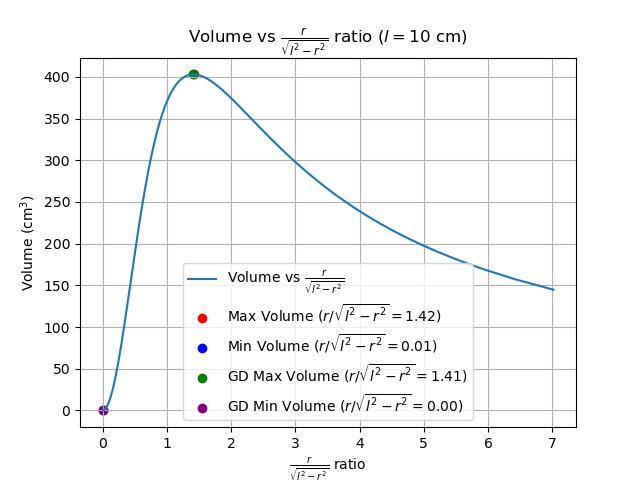
\includegraphics[width=\columnwidth]{figs/fig1.png}
			\caption{Plot of volume versus $r/h$ where $h=\sqrt{l^2-r^2}$}
		\label{stemplot}
	\end{figure}
	
\end{document}  
